% CSC413 Final Project Proposal
% Requires the NeurIPS 2026 style file (neurips_2026.sty) and references.bib in the same folder.
% Easiest: open "Formatting Instructions for NeurIPS 2026" on Overleaf, paste this in, and upload references.bib.
% Search for "TODO" to find every placeholder.

\documentclass{article}
\usepackage[main, final]{neurips_2026}

\usepackage[utf8]{inputenc}
\usepackage[T1]{fontenc}
\usepackage{hyperref}
\usepackage{url}
\usepackage{booktabs}
\usepackage{amsmath}
\usepackage{amsfonts}
\usepackage{microtype}
\usepackage{graphicx}
\usepackage{tikz}
\usetikzlibrary{positioning, arrows.meta}

\title{Rule-Constrained Transformer Generation of Bach-Style Four-Part Chorales}

\author{
  Alan Olegovich Khaev \And
  Saurabh Nair \And
  Kamil Chaudhry \And
  Haris Faisal \\
  University of Toronto Mississauga
}

\begin{document}

\maketitle

\begin{abstract}
We propose a generative sequence model that composes four-part chorales in the style of Johann Sebastian Bach. Given a short musical prefix, represented as a sequence of discrete pitch tokens on a fixed time grid, the model predicts a probability distribution over the next token and generates the continuation autoregressively. Our primary model is a decoder-only Transformer trained with teacher forcing on the Bach chorales in the music21 corpus (approximately 370 pieces; TODO: confirm count). Because this dataset is small by deep learning standards, we apply key transposition as a domain-appropriate data augmentation, which increases the effective training set roughly twelvefold. Inspired by rule-based systems such as Sid Meier's CPU Bach, we additionally apply constrained decoding at generation time: candidate notes that violate basic rules of counterpoint, such as voice ranges and parallel fifths or octaves, are masked before sampling. We compare the Transformer against a first-order Markov chain and an LSTM baseline using held-out negative log-likelihood and the rate of counterpoint rule violations in generated music. This work concerns symbolic music generation, sequence modelling, and constrained decoding.
\end{abstract}

\section{Introduction}

\emph{Musical Counterpoint} is the practice of combining several independent melodic lines, called \emph{voices}, to create a polyphonic texture that carries harmonic meaning within itself, while also being generally pleasing to listen to. The four-part chorales of J.\,S.~Bach (soprano, alto, tenor, and bass) are a standard benchmark for computational music generation because they follow well-documented stylistic rules while still showing substantial variety and a level of compositional complexity few have been able to emulate since Bachs' time. Creating music following the rules of counterpoint has historically been difficult for many musicians, and even more challenging for computers: each voice must form a musically coherent melody on its own, while every simultaneous combination of voices must also satisfy harmonic and structural constraints.

Regarding machine-generated counterpoint, two broad approaches exist. Rule-based systems encode music theory directly and produce well-formed but often predictable music since they often lack the spontaneity and creative decision making capabilities of a human composer. Learned models capture stylistic patterns from data but can produce errors that a trained musician would immediately identify. This project combines the two: a Transformer learns the style from data, and a small set of hard-coded rules removes clear violations during generation. Additionally, a variable degree of randomness or "creativity" may be introduced via \emph{Temperature} which may help break a models' habit of "playing it safe" and take the music into new, unconventional territory (while still conforming to the rules).

Concretely, the input to our model is a variable-length sequence of discrete tokens encoding the first few moments of a chorale (or a \emph{subject} - a short introductory idea for the model to work with), and the output is a continuation of that sequence in the same token format, which is converted back into a playable MIDI file.

A deep learning approach is reasonable here for three reasons. First, the task is naturally a sequence prediction problem in which each note depends on a long musical context, which is the setting Transformers are designed for. Second, prior neural models have produced chorales that listeners struggle to distinguish from Bach's own~\cite{hadjeres2017deepbach, liang2016bachbot}. Third, the rule-violation metric gives an interpretable measure of whether the model has learned musical structure, beyond what likelihood alone reveals. Additional criteria will also be used during the qualitative assessement of the models' performance, as a means to provide a more defined reward signal during training. These metrics are meant to be more high-level, focusing on the outputs' musical structure, form, and general listening enjoyment.

\section{Background and Related Work}

\paragraph{Musical background.} A \emph{MIDI} file stores music as a stream of events, each specifying a pitch (an integer from 0 to 127), a start time, and a duration. It contains all relevant contextual information about a piece in question, such as key, time signature, and tempo. \emph{Conjunct motion} refers to a voice moving in a stepwise manner (short intervals), and \emph{disjunct motion} refers to a voice moving in larger leaps; Baroque melodies favour conjunct motion, but knowing how to use a combination of both is vital to writing good music. \emph{Parallel fifths and octaves} occur when two voices move in the same direction while staying at an interval of fifth or an octave apart; this is a standard rule violation in Bach's style because it makes the voices sound less independent, and is \textbf{entirely forbidden}. A \emph{Markov chain} predicts the next state using only the current state, with transition probabilities estimated from counts.

\paragraph{Rule-based generation.} Sid Meier's CPU Bach (1994) generated Baroque-style polyphony in real time without machine learning. Its approach, described in a US patent~\cite{cpubach}, combined Markov-chain note selection, which favours stepwise motion, with hard-coded structural rules for harmonic progression, modulation, and voice entry. We use this design in two ways: a Markov chain serves as our simplest baseline, and its rule-based component motivates our constrained decoding.

\paragraph{Neural chorale generation.} \citet{liang2016bachbot} trained an LSTM~\cite{hochreiter1997lstm} on Bach chorales and reported that listeners often could not distinguish its output from the originals. \citet{hadjeres2017deepbach} used recurrent networks with Gibbs sampling and allowed user-specified constraints, such as fixed notes, during generation. \citet{huang2017coconet} framed counterpoint as filling in missing notes with a convolutional network, an approach that later powered the 2019 Google Bach Doodle~\cite{huang2019doodle}.

\paragraph{Transformers for music.} The Transformer~\cite{vaswani2017attention} replaces recurrence with self-attention, allowing each position to attend directly to every earlier position. \citet{huang2019music} showed that Transformers capture long-range structure in symbolic music better than LSTMs, which motivates our choice of primary model.

\paragraph{Our contribution.} Prior neural chorale models learn musical rules only implicitly from data, while rule-based systems such as CPU Bach use no learning. Our project combines a Transformer with explicit counterpoint rules applied at decoding time. Unlike the constraints in DeepBach, which fix specific notes chosen by a user, our constraints are general music-theory rules, and we measure directly how often each model violates them with and without the constraints.

\section{Data}

\paragraph{Source.} We use the Bach chorales included in the music21 Python library~\cite{cuthbert2010music21}. Bach's compositions are in the public domain, and the music21 corpus is distributed for research and educational use, which avoids the licensing uncertainty of individually sequenced MIDI files from other websites (TODO: confirm music21 corpus license terms). As a possible extension, we may also use the two-part Inventions and three-part Sinfonias.

\paragraph{Summary statistics.} Table~\ref{tab:stats} reports the key properties of the dataset, and Figure~\ref{fig:explore} shows the distribution of chorale lengths and of pitches in each voice. (TODO: fill in using a short music21 script, and add one or two sentences on what these statistics imply for the difficulty of the task, e.g.\ sequence length relative to model context size.)

\begin{figure}[t]
  \centering
  \fbox{\parbox[c][3.5cm][c]{0.9\linewidth}{\centering TODO: exploratory figure, e.g.\ (left) histogram of chorale lengths in sixteenth-note steps; (right) pitch distribution per voice.}}
  \caption{Exploratory statistics of the Bach chorale dataset. Left: distribution of chorale lengths in sixteenth-note time steps. Right: distribution of MIDI pitches for the soprano, alto, tenor, and bass voices. (TODO: update caption to describe the final figure.)}
  \label{fig:explore}
\end{figure}

\begin{table}[t]
  \centering
  \caption{Summary statistics of the Bach chorale dataset (placeholder values to be filled in).}
  \label{tab:stats}
  \begin{tabular}{lr}
    \toprule
    Statistic & Value \\
    \midrule
    Number of chorales & TODO \\
    Total notes (all voices) & TODO \\
    Mean / max length (sixteenth-note steps) & TODO / TODO \\
    Pitch range: soprano, alto, tenor, bass & TODO \\
    Major / minor key proportion & TODO \\
    Mean sequence length after tokenization & TODO \\
    \bottomrule
  \end{tabular}
\end{table}

\paragraph{Representation.} Each chorale is quantized to a grid of sixteenth-note time steps. At each step we record one token per voice in a fixed order (soprano, alto, tenor, bass). Each token is either a MIDI pitch, a \emph{hold} token indicating that the previous note continues, or a \emph{rest} token. The four voices are interleaved into a single sequence, so that a piece of $T$ time steps becomes a sequence of $4T$ tokens. The vocabulary therefore contains the pitches observed in the data plus the hold, rest, start, and end tokens (TODO: report final vocabulary size). This ordering means that when the model generates a bass note, the soprano, alto, and tenor notes at the same time step are already known, which allows the constraint checks described in Section~\ref{sec:model}.

\paragraph{Cleaning.} We will discard chorales that do not contain exactly four voices and chorales whose note durations cannot be represented on the sixteenth-note grid, and we will report how many pieces each filter removes. (TODO: report counts.)

\paragraph{Augmentation.} Because roughly 370 pieces is small for a Transformer, we transpose each training chorale to every key in which all voices remain within their observed ranges. Transposition preserves musical structure exactly, so it is an appropriate augmentation for this domain.

\paragraph{Split.} We split by chorale into 80\% training, 10\% validation, and 10\% test sets, so that test pieces are never seen in any form during training. Transposition is applied only after splitting, to prevent transposed copies of test pieces from leaking into the training set.

\section{Model Architecture}
\label{sec:model}

\paragraph{Primary model.} Figure~\ref{fig:arch} illustrates the overall system. Our main model is a decoder-only Transformer. Each input token is mapped to a learned embedding, to which we add a learned positional embedding and a learned voice embedding indicating which of the four voices the token belongs to. The sequence then passes through a stack of masked self-attention layers, each followed by a position-wise feed-forward network, with residual connections and layer normalization. A causal mask ensures that each position attends only to earlier positions. A final linear layer and softmax produce a distribution over the vocabulary for the next token. We train with teacher forcing, minimizing the cross-entropy between predicted distributions and the true next tokens. As a starting configuration we plan to use 6 layers, a model dimension of 256, and 4 attention heads (approximately 5 million parameters), and we will tune these values on the validation set. All models will be implemented in PyTorch~\cite{paszke2019pytorch}, with music21 used for parsing and MIDI export.

\paragraph{Constrained decoding.} During generation, before sampling each token, we set the probability of every candidate token that violates a rule to zero and renormalize the remaining distribution. The initial rule set is (1) each voice must stay within its typical range, (2) no parallel fifths or octaves between any pair of voices, and (3) no voice crossing, meaning a lower voice may not sound above a higher one. These rules are applied only at generation time, so the trained model is unchanged and we can measure the effect of the constraints directly.

\paragraph{Baselines.} We compare against (1) a first-order Markov chain over the same token vocabulary, which mirrors CPU Bach's note-level method, and (2) a single-layer LSTM of comparable parameter count trained with the same objective. If the Transformer does not outperform the Markov chain on held-out likelihood, we will treat that as evidence that the model has failed to learn useful structure.

\paragraph{Evaluation.} We will report (1) per-token negative log-likelihood on the test set, (2) the percentage of generated time steps that violate each rule, with and without constrained decoding, and (3) the distance between pitch-class distributions of generated and real chorales. We will also present selected generated excerpts for qualitative analysis.

\begin{figure}[t]
  \centering
  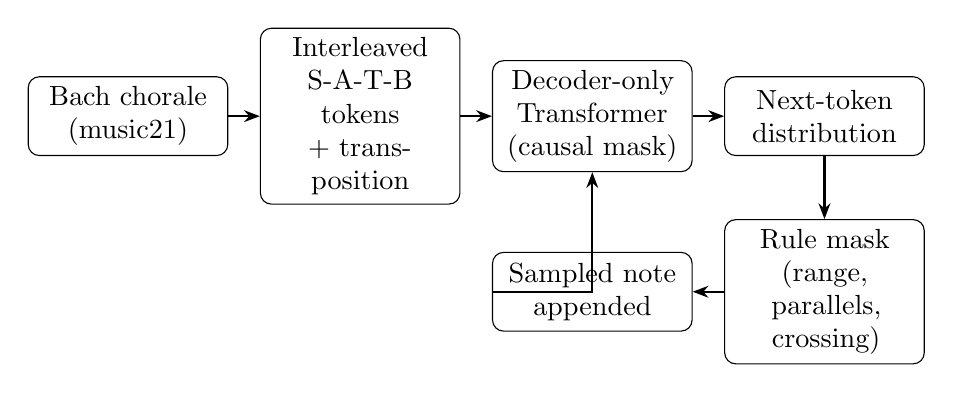
\begin{tikzpicture}[
      box/.style={draw, rounded corners, align=center, minimum height=1cm, text width=2.3cm},
      arr/.style={-{Stealth[length=2mm]}, thick}
    ]
    \node[box] (midi) {Bach chorale\\(music21)};
    \node[box, right=0.4cm of midi] (tok) {Interleaved\\S-A-T-B tokens\\+ transposition};
    \node[box, right=0.4cm of tok] (tf) {Decoder-only\\Transformer\\(causal mask)};
    \node[box, right=0.4cm of tf] (soft) {Next-token\\distribution};
    \node[box, below=0.8cm of soft] (mask) {Rule mask\\(range, parallels,\\crossing)};
    \node[box, left=0.4cm of mask] (sample) {Sampled note\\appended};
    \draw[arr] (midi) -- (tok);
    \draw[arr] (tok) -- (tf);
    \draw[arr] (tf) -- (soft);
    \draw[arr] (soft) -- (mask);
    \draw[arr] (mask) -- (sample);
    \draw[arr] (sample.west) -| (tf.south);
  \end{tikzpicture}
  \caption{Overview of the proposed system. Chorales are converted into a single token sequence that interleaves the soprano, alto, tenor, and bass voices. A decoder-only Transformer predicts a distribution over the next token, a rule mask removes tokens that would break counterpoint rules, and the sampled token is appended to the input for the next step.}
  \label{fig:arch}
\end{figure}

\section{Ethical Considerations}

\paragraph{Data provenance.} Although Bach's compositions are in the public domain, a specific digital transcription can be the copyrighted work of the person who produced it. We therefore use a corpus distributed for research use rather than collecting MIDI files from arbitrary websites.

\paragraph{Transfer to living artists.} The pipeline we build is independent of the composer. Applied to the work of living musicians without consent, the same method would raise the copyright and compensation concerns at the centre of current disputes over commercial music generators.

\paragraph{Misattribution.} The attribution of Baroque works is not fully settled: several pieces once credited to Bach have been reassigned to other composers. Generated pieces presented as rediscovered or newly attributed works could mislead listeners and scholars, so all output from this project will be clearly labelled as machine-generated.

\paragraph{Economic impact.} Systems that generate stylistically correct music cheaply compete most directly with composers of stock, library, and educational music, who are often less established than the artists usually discussed in this debate.

\paragraph{Cultural bias.} Our rules and data encode one Western tradition's conventions as correct. A model or metric that treats these conventions as universal would misjudge music from other traditions, which matters if similar tools are used in education or assessment.

\section{Work Division}

Work is divided by stage of the pipeline, so that each member owns one component and the handoffs between components are clearly defined. Table~\ref{tab:work} lists each member's responsibilities and estimated weekly time commitment. Each member also writes the report section describing their component, and a second member edits it. (TODO: adjust names and hours.)

\begin{table}[t]
  \centering
  \caption{Division of work and estimated hours per member in each of the four project weeks.}
  \label{tab:work}
  \small
  \begin{tabular}{p{1.9cm}p{6.4cm}cccc}
    \toprule
    Member & Responsibilities & Wk 1 & Wk 2 & Wk 3 & Wk 4 \\
    \midrule
    Alan & Token representation design; rule checker and constrained decoding; music-theory background; qualitative analysis of generated samples. & 6 & 5 & 5 & 4 \\
    Saurabh & Transformer implementation and training loop; overfitting a single chorale; hyperparameter tuning; training curves; parameter count and architecture figure. & 3 & 7 & 7 & 3 \\
    Kamil & Data loading, cleaning, and tokenization; summary statistics; transposition augmentation; data split; README and code documentation. & 8 & 4 & 3 & 5 \\
    Haris & Markov chain and LSTM baselines; evaluation scripts (likelihood, rule-violation rate, pitch-class distance); results tables; final report assembly. & 3 & 6 & 6 & 5 \\
    \bottomrule
  \end{tabular}
\end{table}

\paragraph{Dependencies.} Alan and Member 3 agree on the token format jointly in the first two days, since every later component depends on it. Member 3 delivers a preliminary tokenized dataset by the end of week 1, so that the Transformer and baselines can begin training before cleaning is finalized. Saurabh and Member 4 share a single training and evaluation interface, so that all models are compared under identical conditions. If a component falls behind, the member responsible for the downstream component assists through pair programming.

\paragraph{Collaboration.} The team meets weekly (TODO: day and time, e.g.\ Tuesdays 4--5 pm) to review progress against the timeline below, and coordinates between meetings through a group chat and a shared GitHub repository, with changes merged through pull requests reviewed by one other member.

\paragraph{Timeline.}
\textbf{Week 1:} data pipeline and statistics complete; Markov baseline trained; Transformer overfits a single chorale.
\textbf{Week 2:} full Transformer and LSTM training; rule checker implemented.
\textbf{Week 3:} hyperparameter tuning; constrained decoding integrated; evaluation run.
\textbf{Week 4:} analysis, figures, README, and report writing.
(TODO: align with actual course deadlines.)

\bibliographystyle{plainnat}
\bibliography{references}

\end{document}